%%%%%%%%%%%%%%%%%%%%%%%%%%%%%%%%%%%%%%%%%
% Programming/Coding Assignment
% LaTeX Template
%
% This template has been downloaded from:
% http://www.latextemplates.com
%
% Original author:
% Ted Pavlic (http://www.tedpavlic.com)
%
% Note:
% The \lipsum[#] commands throughout this template generate dummy text
% to fill the template out. These commands should all be removed when 
% writing assignment content.
%
% This template uses a Python script as an example snippet of code, most other
% languages are also usable. Configure them in the "CODE INCLUSION 
% CONFIGURATION" section.
%
%%%%%%%%%%%%%%%%%%%%%%%%%%%%%%%%%%%%%%%%%

%----------------------------------------------------------------------------------------
%	PACKAGES AND OTHER DOCUMENT CONFIGURATIONS
%----------------------------------------------------------------------------------------

\documentclass{article}

\usepackage{fancyhdr} % Required for custom headers
\usepackage{lastpage} % Required to determine the last page for the footer
\usepackage{extramarks} % Required for headers and footers
\usepackage[usenames,dvipsnames]{color} % Required for custom colors
\usepackage{graphicx} % Required to insert images
\usepackage{listings} % Required for insertion of code
\usepackage{courier} % Required for the courier font
\usepackage{lipsum} % Used for inserting dummy 'Lorem ipsum' text into the template
\usepackage{microtype}
\usepackage[reqno]{amsmath}
%\usepackage{amsmath}
\usepackage{amsfonts}
\usepackage{amssymb}
\usepackage[utf8]{inputenc}
\usepackage{booktabs} 
\usepackage{subfig}
\usepackage{textcomp} 
\usepackage[dvipsnames]{xcolor}
\usepackage[pdftex,bookmarks,colorlinks,breaklinks]{hyperref}
\usepackage[outdir=./]{epstopdf}
\usepackage{cleveref}
\graphicspath{{/Users/michaeljaquier/Documents/int/BMN/miniproject/res/}}
% Margins
\topmargin=-0.45in
\evensidemargin=0in
\oddsidemargin=0in
\textwidth=6.5in
\textheight=9.0in
\headsep=0.25in

\linespread{1.1} % Line spacing

% Set up the header and footer
\pagestyle{fancy}
\lhead{\hmwkAuthorName} % Top left header
\chead{ \hmwkTitle} % Top center head
\rhead{\firstxmark} % Top right header
\lfoot{\lastxmark} % Bottom left footer
\cfoot{} % Bottom center footer
\rfoot{Page\ \thepage\ of\ \protect\pageref{LastPage}} % Bottom right footer
\renewcommand\headrulewidth{0.4pt} % Size of the header rule
\renewcommand\footrulewidth{0.4pt} % Size of the footer rule

\setlength\parindent{0pt} % Removes all indentation from paragraphs
\newcommand\myshade{85}
\colorlet{mylinkcolor}{NavyBlue}
\colorlet{mycitecolor}{YellowOrange}
\colorlet{myurlcolor}{violet}
\hypersetup{
	linkcolor  = mylinkcolor!\myshade!black,
	citecolor  = mycitecolor!\myshade!black,
	urlcolor   = myurlcolor!\myshade!black,
	colorlinks = true}


%----------------------------------------------------------------------------------------
%	CODE INCLUSION CONFIGURATION
%----------------------------------------------------------------------------------------

\definecolor{MyDarkGreen}{rgb}{0.0,0.4,0.0} % This is the color used for comments
\lstloadlanguages{Python} % Load Python syntax for listings, for a list of other languages supported see: ftp://ftp.tex.ac.uk/tex-archive/macros/latex/contrib/listings/listings.pdf
\lstset{language=Python, % Use Python in this example
        frame=single, % Single frame around code
        basicstyle=\small\ttfamily, % Use small true type font
        keywordstyle=[1]\color{Blue}\bf, % Python functions bold and bluex
        keywordstyle=[2]\color{Purple}, % Python function arguments purple
        keywordstyle=[3]\color{Blue}\underbar, % Custom functions underlined and blue
        identifierstyle=, % Nothing special about identifiers                                         
        commentstyle=\usefont{T1}{pcr}{m}{sl}\color{MyDarkGreen}\small, % Comments small dark green courier font
        stringstyle=\color{Purple}, % Strings are purple
        showstringspaces=false, % Don't put marks in string spaces
        tabsize=2, % 5 spaces per tab
        %
        % Put standard Python functions not included in the default language here
        morekeywords={rand},
        %
        % Put Python function parameters here
        morekeywords=[2]{on, off, interp},
        %
        % Put user defined functions here
        morekeywords=[3]{test},
       	%
        morecomment=[l][\color{Blue}]{...}, % Line continuation (...) like blue comment
        numbers=left, % Line numbers on left
        firstnumber=1, % Line numbers start with line 1
        numberstyle=\tiny\color{Blue}, % Line numbers are blue and small
        stepnumber=5 % Line numbers go in steps of 5
}

% Creates a new command to include a perl script, the first parameter is the filename of the script (without .pl), the second parameter is the caption
\newcommand{\pythonscript}[2]{
\begin{itemize}
\item[]\lstinputlisting[caption=#2,label=#1]{#1.py}
\end{itemize}
}

%----------------------------------------------------------------------------------------
%	DOCUMENT STRUCTURE COMMANDS
%	Skip this unless you know what you're doing
%----------------------------------------------------------------------------------------

% Header and footer for when a page split occurs within a problem environment
\newcommand{\enterProblemHeader}[1]{
\nobreak\extramarks{#1}{#1 continued on next page\ldots}\nobreak
\nobreak\extramarks{#1 (continued)}{#1 continued on next page\ldots}\nobreak
}

% Header and footer for when a page split occurs between problem environments
\newcommand{\exitProblemHeader}[1]{
\nobreak\extramarks{#1 (continued)}{#1 continued on next page\ldots}\nobreak
\nobreak\extramarks{#1}{}\nobreak
}

\setcounter{secnumdepth}{0} % Removes default section numbers
\newcounter{homeworkProblemCounter} % Creates a counter to keep track of the number of problems

\newcommand{\homeworkProblemName}{}
\newenvironment{homeworkProblem}[1][Problem \arabic{homeworkProblemCounter}]{ % Makes a new environment called homeworkProblem which takes 1 argument (custom name) but the default is "Problem #"
\stepcounter{homeworkProblemCounter} % Increase counter for number of problems
\renewcommand{\homeworkProblemName}{#1} % Assign \homeworkProblemName the name of the problem
\section{\homeworkProblemName} % Make a section in the document with the custom problem count
\enterProblemHeader{\homeworkProblemName} % Header and footer within the environment
}{
\exitProblemHeader{\homeworkProblemName} % Header and footer after the environment
}

\newcommand{\problemAnswer}[1]{ % Defines the problem answer command with the content as the only argument
\noindent\framebox[\columnwidth][c]{\begin{minipage}{0.98\columnwidth}#1\end{minipage}} % Makes the box around the problem answer and puts the content inside
}

\newcommand{\homeworkSectionName}{}
\newenvironment{homeworkSection}[1]{ % New environment for sections within homework problems, takes 1 argument - the name of the section
\renewcommand{\homeworkSectionName}{#1} % Assign \homeworkSectionName to the name of the section from the environment argument
\subsection{\homeworkSectionName} % Make a subsection with the custom name of the subsection
\enterProblemHeader{\homeworkProblemName\ [\homeworkSectionName]} % Header and footer within the environment
}{
\enterProblemHeader{\homeworkProblemName} % Header and footer after the environment
}

%----------------------------------------------------------------------------------------
%	NAME AND CLASS SECTION
%----------------------------------------------------------------------------------------

\newcommand{\hmwkTitle}{Miniproject\  Single Neuron} % Assignment title
\newcommand{\hmwkDueDate}{Monday,\ January\ 1,\ 2012} % Due date
\newcommand{\hmwkClass}{Biological Modeling of Neural Networks} % Course/class
\newcommand{\hmwkClassTime}{10:30am} % Class/lecture time
\newcommand{\hmwkClassInstructor}{Jones} % Teacher/lecturer
\newcommand{\hmwkAuthorName}{Michael Jaquier} % Your name

%----------------------------------------------------------------------------------------
%	TITLE PAGE
%----------------------------------------------------------------------------------------

\title{
\vspace{2in}
\textmd{\textbf{\hmwkClass:\ \hmwkTitle}}\\
%\normalsize\vspace{0.1in}\small{Due\ on\ \hmwkDueDate}\\
%\vspace{0.1in}\large{\textit{\hmwkClassInstructor\ \hmwkClassTime}}
\vspace{3in}
}

\author{\textbf{\hmwkAuthorName}}
\date{} % Insert date here if you want it to appear below your name

%----------------------------------------------------------------------------------------

\begin{document}

\maketitle

%----------------------------------------------------------------------------------------
%	TABLE OF CONTENTS
%----------------------------------------------------------------------------------------

%\setcounter{tocdepth}{1} % Uncomment this line if you don't want subsections listed in the ToC

\newpage
\tableofcontents
\newpage

%----------------------------------------------------------------------------------------
% INTRO
%----------------------------------------------------------------------------------------

\begin{homeworkProblem}[Introduction]
In order to establish our base model we utilize the Brian2 with a set of standard Hodgkin Huxley (HH) equations in order to establish an ideal neuron. We build upon the standard model of membrane potentials with two ion channels. 
\begin{equation}\label{e1}
\frac{dV}{dt} = (I_{ext} + g_{Na}(E_{Na} - V) + g_{K}(E_{K} - V) + g_{l}(E_{l} - V))/C_{m},
\end{equation}
where $E_{ion}$ are the reversal potentials of each ion, $E_{l}$ is the leak present in the membrane. Conductances - $g_{Ion}$ for a given channel are modulated in the HH model by empirically determined parameters, $g_{K} = \tilde{g}_{K}n^4$ and $g_{Na} = \tilde{g}_{Na}m^3h$. Other parameters are tuned in order to facilitate a resting potential of 0mV for ease of calculations. 

Ion channel dynamics ($x_{\infty}(V)$, $\tau_{x}(V)$) with $x\in \left\lbrace m,h,n\right\rbrace $, channel dynamics are modeled from a series of differential equations built upon the following
\begin{equation}\label{e2}
dx/dt = -\frac{1}{\tau_{x}(V)}(x - x_{\infty}(V)),
\end{equation}
We reparameterize the dynamic equations in order to simplify overall calculations with the following
\begin{equation}\label{e3}
x_{\infty}(V) = \frac{\alpha_{x}(V)}{\alpha_{x}(V) + \beta_{x}(V)},
\end{equation}

\begin{equation}\label{e4}
\tau_{x}(V) = \frac{1}{\alpha_{x}(V) + \beta_{x}(V)}.
\end{equation}
We utilize equation \ref{e3} and \ref{e4}, with parameters in the appendix, in order to rewrite the dynamics once more and write our neuron into Brian2 as
\begin{equation}\label{e5}
\frac{dx}{dt} = (1 - x)\alpha_{x}(V) - x\beta_{x}(V)
\end{equation}
%Listing \ref{../src/ff1} shows a Python script.
%\pythonscript{../src/ff1}{Sample Python Script With Highlighting}

%----------------------------------------------------------------------------------------
%	PROBLEM 1
%----------------------------------------------------------------------------------------

% To have just one problem per page, simply put a \clearpage after each problem
\begin{homeworkProblem}[Problem 1]
\begin{figure}
\centering
	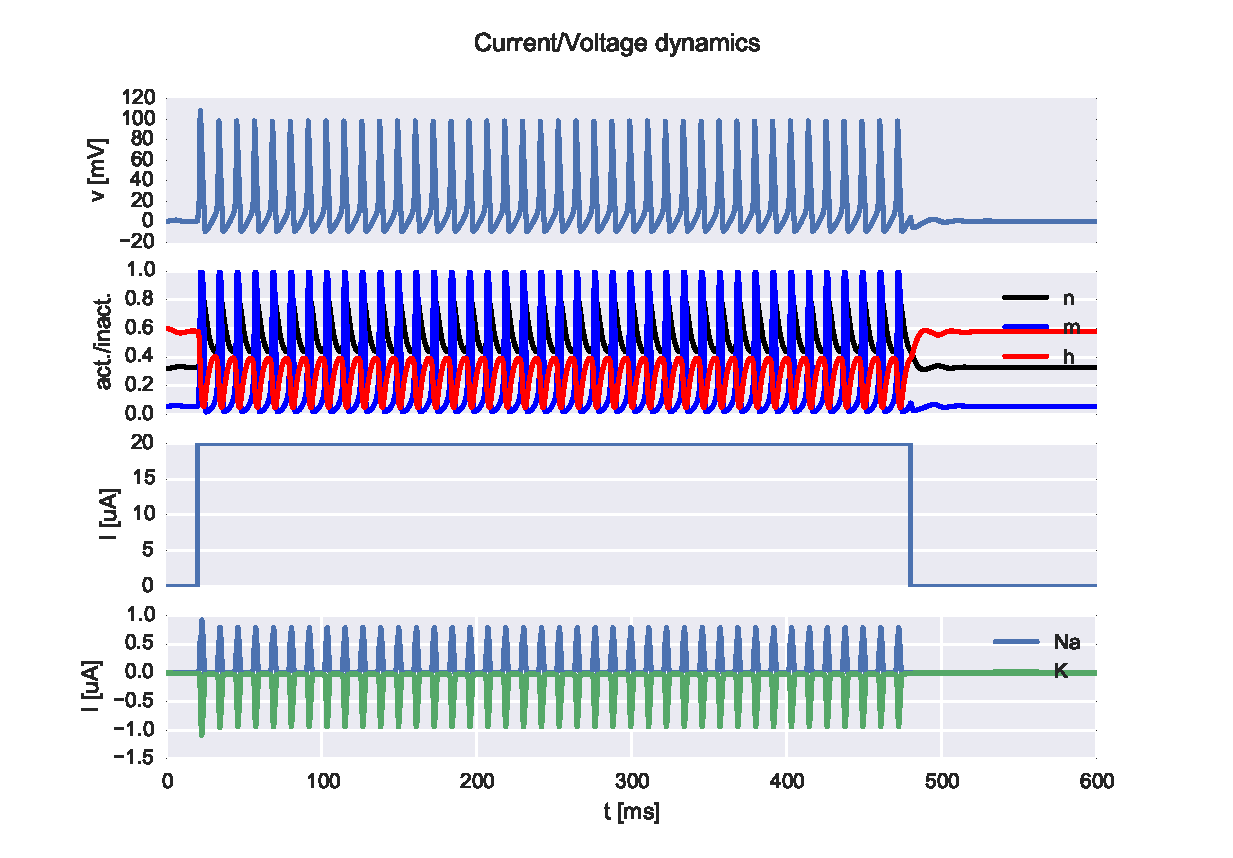
\includegraphics[width=0.9\columnwidth]{normal/c_v_dyn_mhn.eps} % Example image
	\caption{20ms step current input into neuron. From top to bottom:  Voltage trace with two spikes. Dynamic gating variables (n,m and h). Input step current. Sodium and potassium currents.}
\label{c_v}
		\end{figure}
\begin{figure}
		\centering
		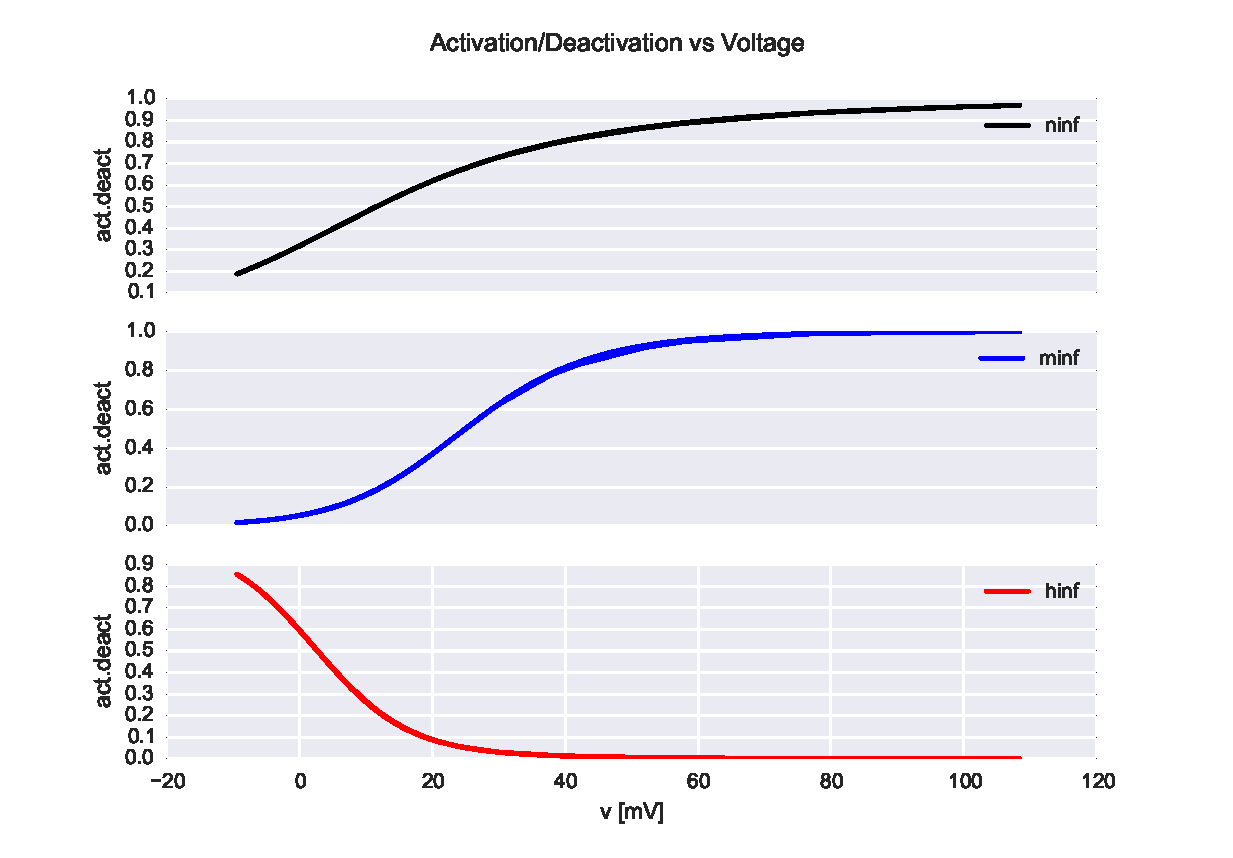
\includegraphics[width=0.9\columnwidth]{normal/act_deact_vs_voltage.eps} % Example image
		\caption{Gating variables ($m_{\infty}$, $n_{\infty}$, $h_{\infty}$) with increasing voltage.}
			\label{inf}
		\end{figure}
\begin{figure}
	\centering
	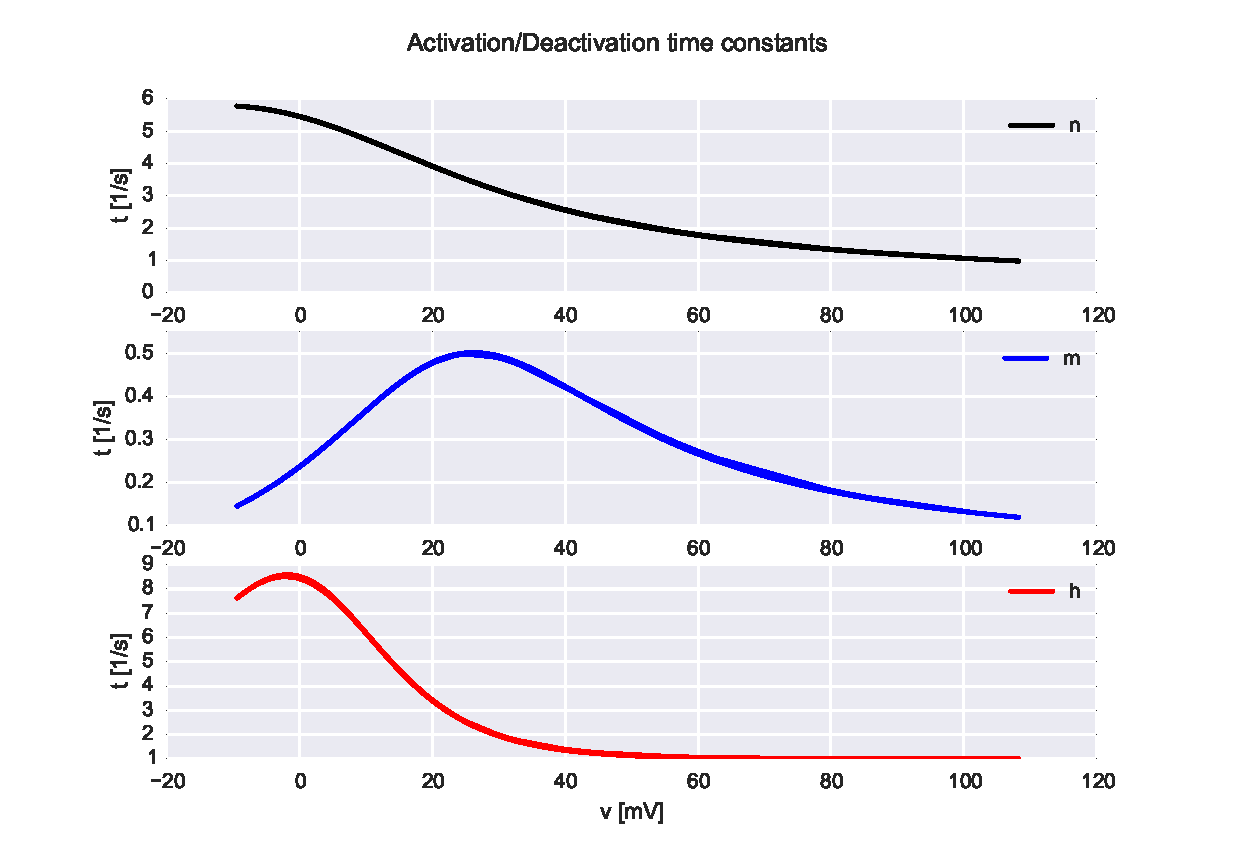
\includegraphics[width=0.9\columnwidth]{normal/tau_plot_act_deact.eps} % Example image
	\caption{Time constants ($\tau_{n}$, $\tau_{m}$, $\tau_{h}$) with increasing voltage.}
	\label{tau}
		\end{figure}
\begin{figure}
	\centering
	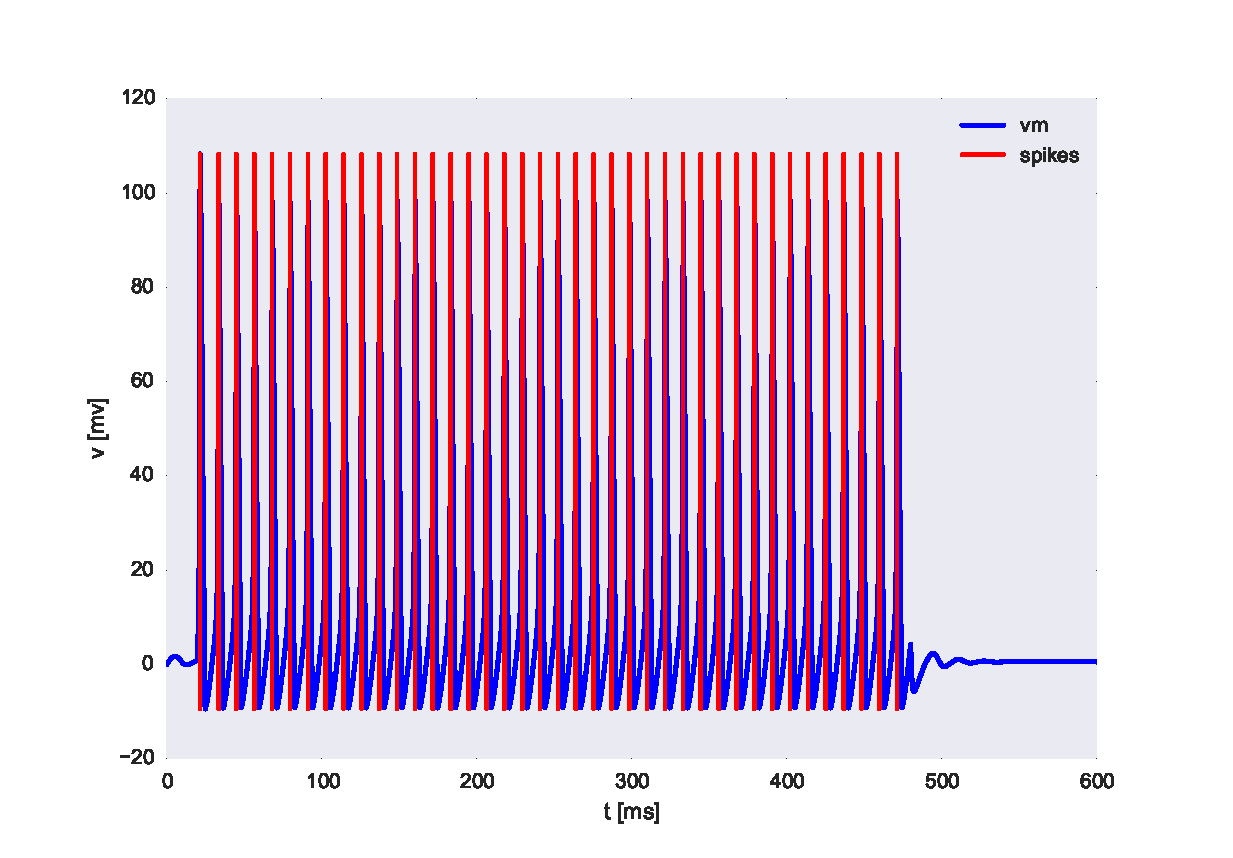
\includegraphics[width=0.9\columnwidth]{normal/VoltageTraceandSpikePoints.eps} % Example image
	\caption{Spike detection algorithm on 20ms voltage trace. Red lines indicate spikes detected by algorithm.}
	\label{spikes}
\end{figure}
\begin{figure}
		\centering
		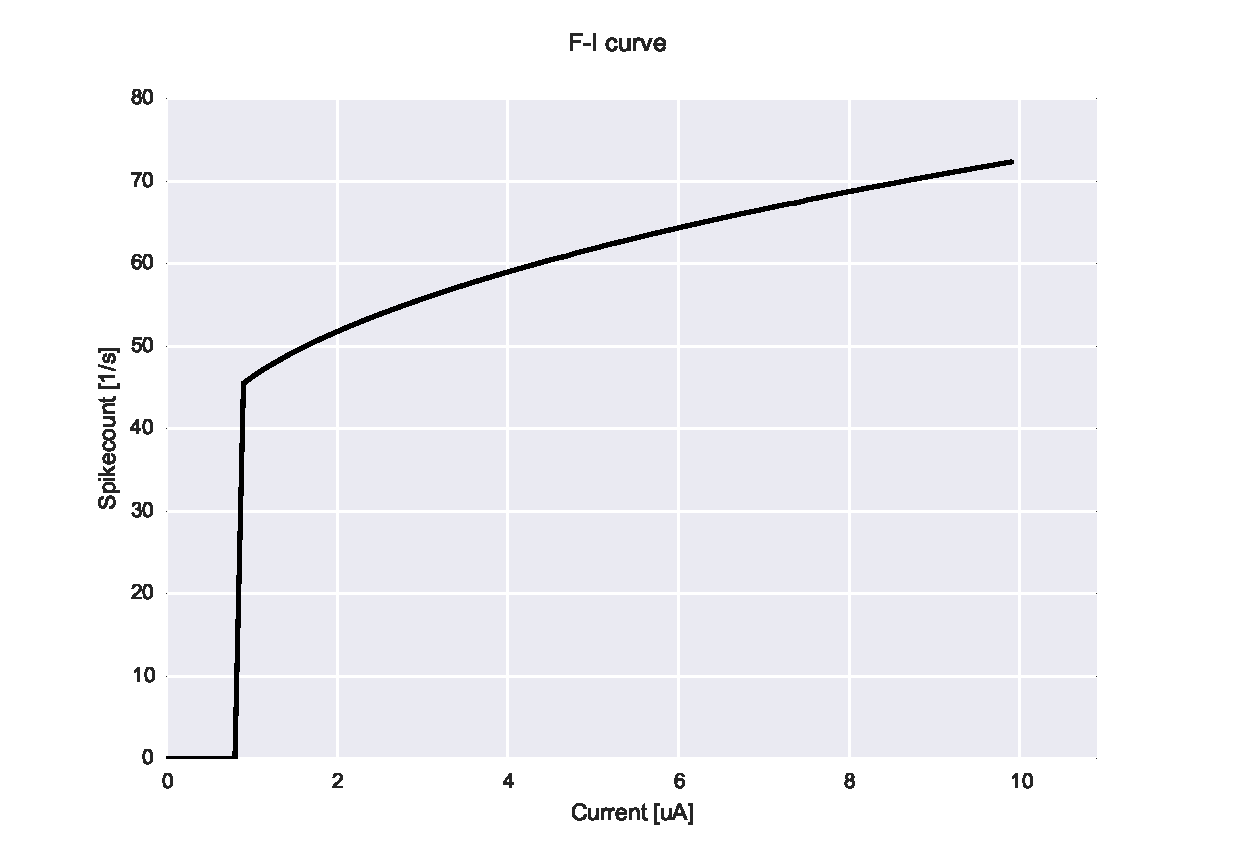
\includegraphics[width=0.9\columnwidth]{normal/f_i_curve.eps} % Example image
		\caption{Frequency - Current curve of neuron as calculated by spike detection algorithm.}
			\label{f_i}
		\end{figure}

A non adapting model is implemented with parameters as per (listing \ref{../alternate/bmnn/HHmodel/hhnorm}.)  With lines 1-10 the setup parameters, lines 12-35 the differential equations used to model the non-adapting neuron. Neuron behavior is plotted in (fig.\ref{c_v}), the dynamic variables ($m$, $n$, and $h$) are responsible for the spike firing. Initially the Na channel gating variables ($m$,$h$) are responsible for both the rapid opening ($m$) of the channel, generating a rapid depolarization, and the delayed deactivation ($h$) of the ion channel which subsequently hyperpolarizes the neuron. Potassium gating variable ($n$) is responsible for activation of the K channel which hyperpolarizes the neuron. 

\subsection{1.1}
The dynamic variables at steady state ($m_{\infty}$, $n_{\infty}$, $h_{\infty}$) serve to elucidate the mechanism that underlies steady firing (fig.\ref{inf}). Of particular interest is the voltage response of the K channel $n$, and Na channel $h$, as the K channel is activate the Na channel deactivates.

The gating variables are additionally tuned by their individual time constants  ($\tau_{n}$, $\tau_{m}$, $\tau_{h}$, fig.\ref{tau}), as can be noted the $m$ dynamic variable responsible for the explosive depolarization of the neuron is significantly quicker than the other time constants whose time scales are fairly similar. The separation of time scales facilitates the normal spiking behavior of the neuron model.
\subsection{1.2}
Spike times are extrapolated via a simple algorithm which evaluates the maximum voltage and determines the index of any voltage value which is within $75\%$  of the computed max (listing \ref{../alternate/bmnn/analysis/spiker}). An example of the spike algorithm is presented in (fig.\ref{spikes}), red lines are detected spikes overlaid on a voltage trace.

\subsection{1.3}
The frequency-current curve (fig.\ref{f_i}) is calculated by applying our spike timing algorithm (listing \ref{../alternate/bmnn/analysis/spiker}) which is applied multiple times across a range of input currents in order to build up the curve. From (fig.\ref{f_i}) the neuron is demonstratively Type II, this is established from its sudden rapid increase in spiking at a fixed point followed by a steady increase up to a maximum firing rate. 	
	
	\clearpage
\end{homeworkProblem}

%----------------------------------------------------------------------------------------
%	PROBLEM 2
%----------------------------------------------------------------------------------------

\begin{homeworkProblem}[Problem 2]
A adaptive neuron is built upon the previous non-adapting model by the addition of a slow potassium ion channel. Given a long enough current input the hyper polarizing effect of the new ion channel slows, and eventually stops, the regular firing pattern of the neuron. Parameters and equations are presented (listing \ref{../alternate/bmnn/HHmodel/hhadap}) note that the base model utilized in the non-adapting model (listing \ref{../alternate/bmnn/HHmodel/hhnorm})  with the addition of the following equations
\begin{equation}\label{w}
\frac{dw}{dt} = \frac{w_{\infty} - w}{tau_{w}},
\end{equation}
\begin{equation}\label{winf}
w_{\infty} = \frac{1}{1+\exp{-3.5\cdot.1}},
\end{equation}
\begin{equation}\label{wtau}
w_{\tau} = \frac{11.4\cdot1000}{3.3\cdot\exp{1.75+0.05}+\exp{-1.75-0.05}},
\end{equation}
units are omitted from the equations for brevity. The new channel conductance is $\tilde{g} = g_{K_{Slow}}w$. The slow $\tau_{w}$ facilitates a delayed inactivation of the channel by hyper polarizing K current after sufficient time.

The adaption inducing channel functions by 'remembering' previous inputs (fig.\ref{a_dyn}), with each subsequent inputs the $w$ dynamic variable increases, thereby opening the channel further with each subsequent action potential. The capacity to remember previous inputs is a result of the significantly longer time constant of $w$ (fig.\ref{a_tau}) results in negligible decay between inputs. 

Further we note the near complete activation of the channel at voltages above resting potential (fig.\ref{actdeac_a}) the channel is very sensitive to any change in voltage, immediately beginning to hyper polarize the cell. A long time constant, together with the lower conductance parameter $g_{M}$ ensures that the neuron still exhibits regular firing patterns. 

Exploring the new spiking behavior of the adapting neuron reveals that the f-i curve is fairly similar to the ideal Type II with the notable exception of oscillations in the spiking rate that are present until the current input reaches some high enough threshold (fig.\ref{a_f_i}). The adaption phenomena is illustrated in more detail (fig.\ref{a_spike}) the behavior exhibited serves to illumine the odd oscillations at lower currents. As can be seen at below a certain threshold (aprox.\ $20\mu A$) the depolarization effect of the slow K channel eventually inhibits any spiking of the neuron after sufficient time. Neuron models compared side by side (fig.\ref{twospike}) demonstrate the adapting mechanism of the new neuron model.


\begin{figure}
	\centering
	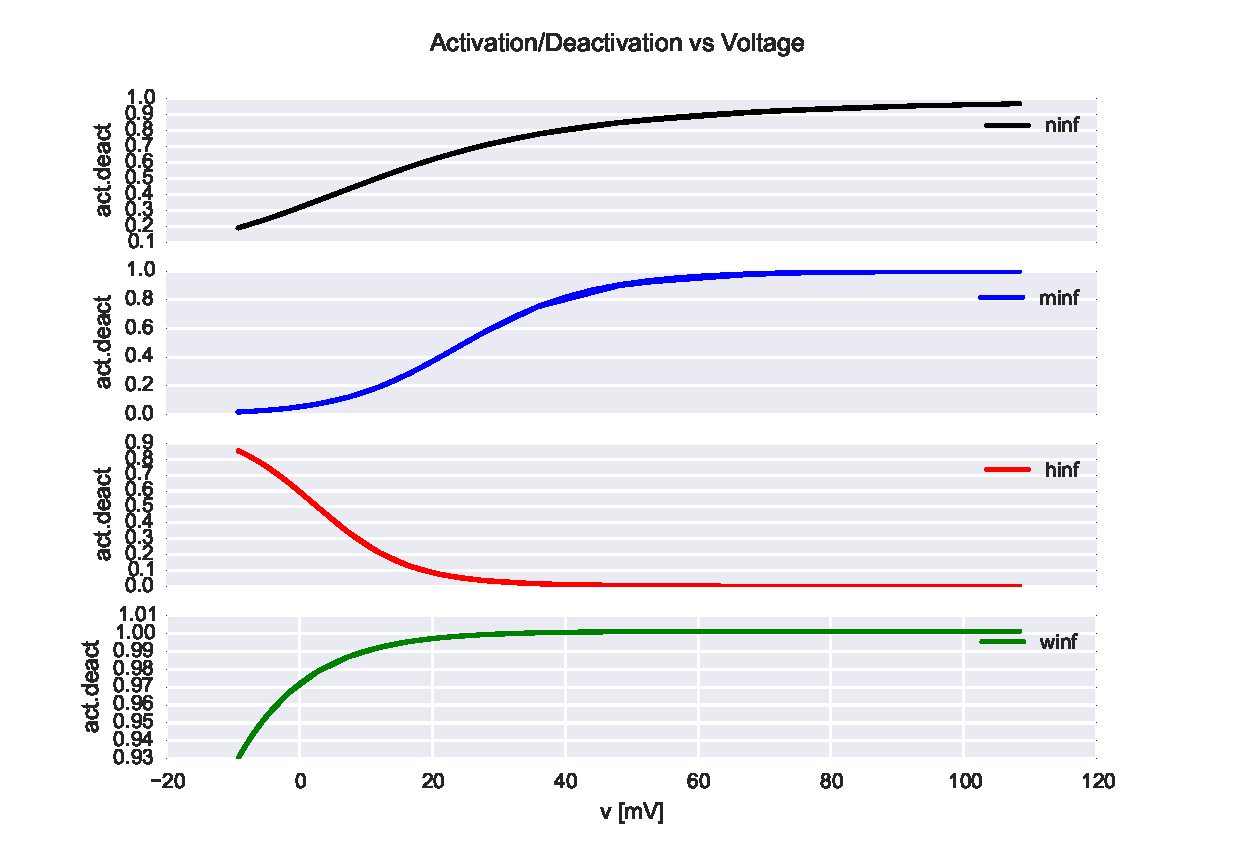
\includegraphics[width=0.9\columnwidth]{adapt/act_deact_vs_voltage_a.eps} % Example image
	\caption{Gating variables ($m_{\infty}$, $n_{\infty}$, $h_{\infty}$, $w_{\infty}$) with increasing voltage.}
	\label{actdeac_a}
\end{figure}
\begin{figure}
	\centering
	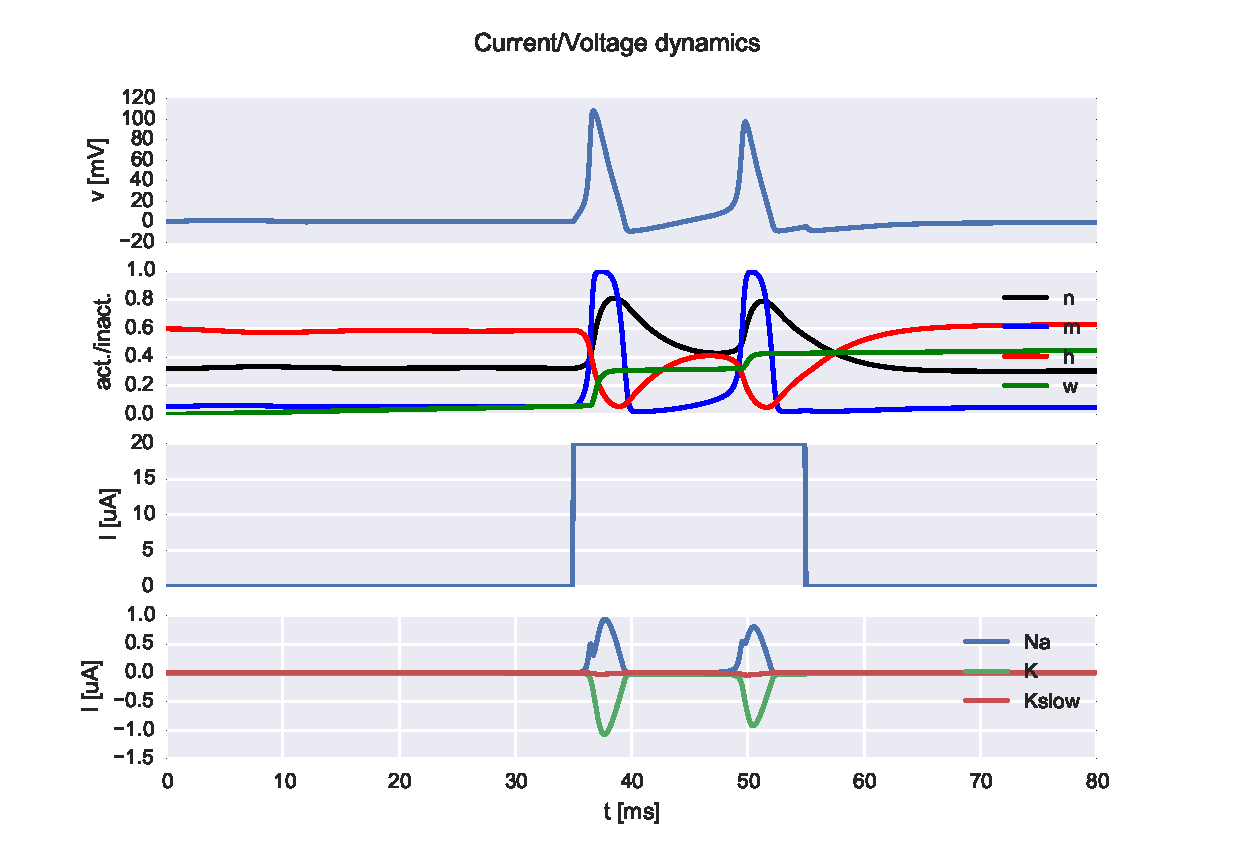
\includegraphics[width=0.9\columnwidth]{adapt/current_voltage_dyn_a.eps} % Example image
	\caption{20ms step current input into adapting neuron. From top to bottom:  Voltage trace with two spikes. Dynamic gating variables (n,m,h,w). Input step current. Sodium, standard potassium current, and slow potassium current.}
	\label{a_dyn}
\end{figure}
\begin{figure}
	\centering
	\includegraphics[width=0.9\columnwidth]{adapt/f_i_curve_a.eps} % Example image
	\caption{Frequency - Current curve of adapting neuron as calculated by spike detection algorithm.}
	\label{a_f_i}
\end{figure}
\begin{figure}
	\centering
	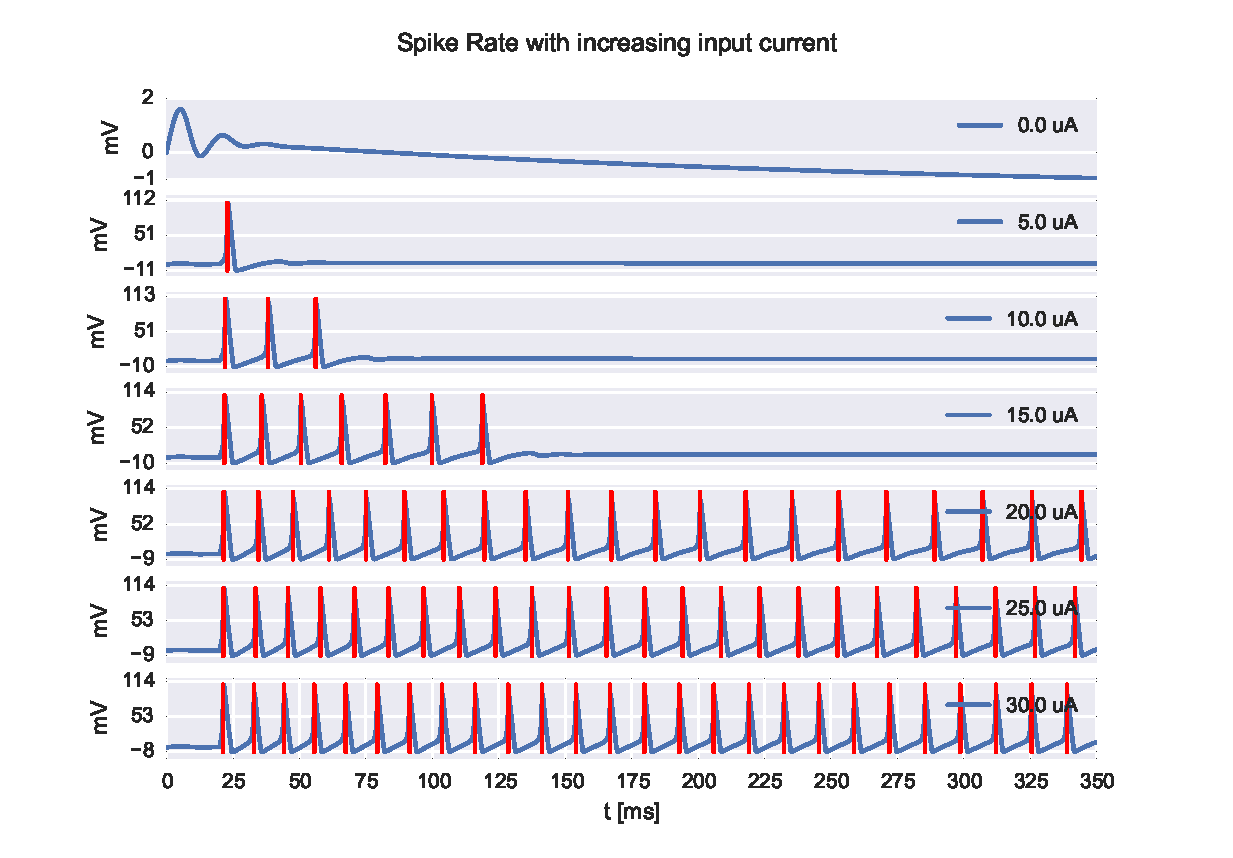
\includegraphics[width=0.9\columnwidth]{adapt/spikerate_inc_current_a.eps} % Example image
	\caption{Change in spiking frequency with increasing current input. Note the increased time between spikes as adaptive parameters activate.}
	\label{a_spike}
\end{figure}
\begin{figure}
	\centering
	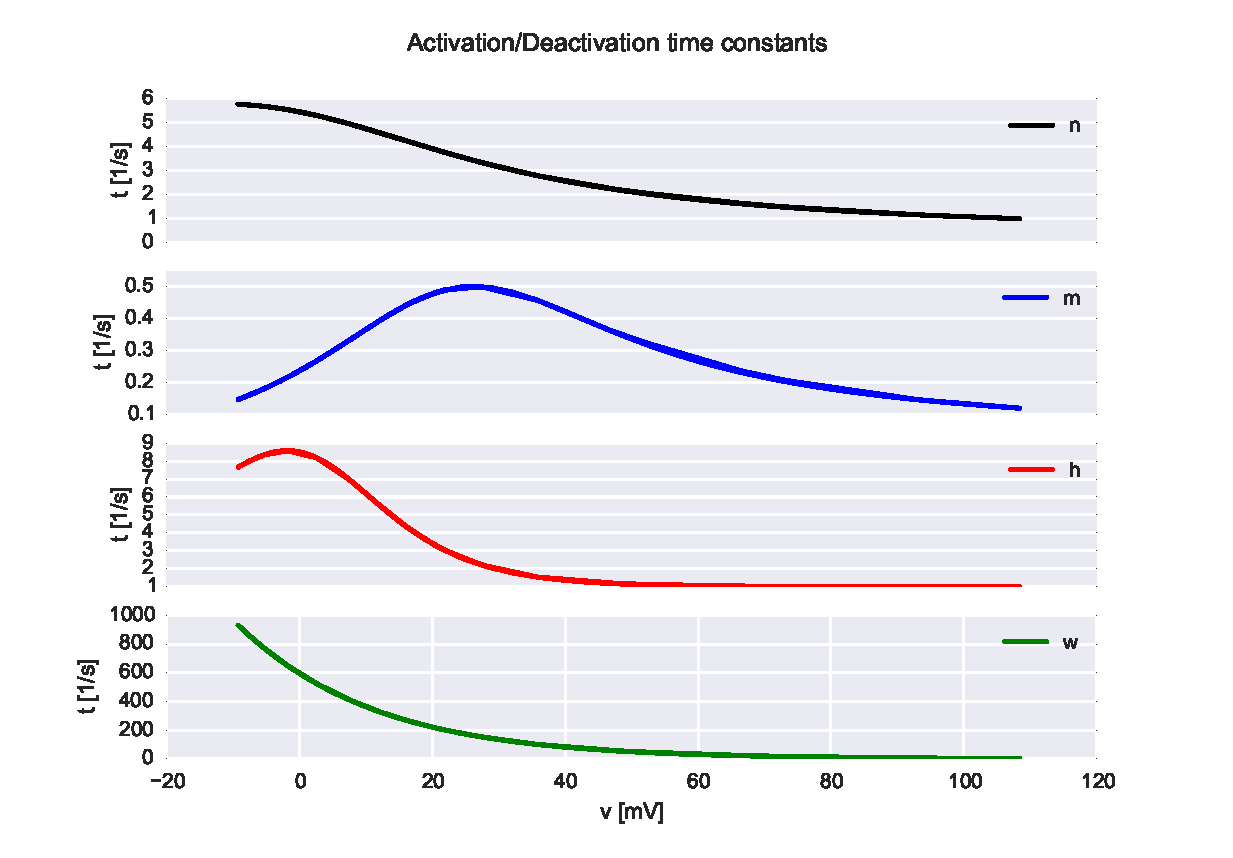
\includegraphics[width=0.9\columnwidth]{adapt/tau_plot_act_deact_a.eps} % Example image
	\caption{Time constants ($\tau_{n}$, $\tau_{m}$, $\tau_{h}$, $\tau_{w}$) with increasing voltage. Note the large separation in time scales between $\tau_{w}$ and other $\tau$ values.}
	\label{a_tau}
\end{figure}
\begin{figure}
	\centering
	\includegraphics[width=0.9\columnwidth]{adapt/twoSpike.eps} % Example image
	\caption{Voltage trace of non-adapting neuron (top) and adapting neuron (bottom) during a 200ms step-current input.}
	\label{twospike}
\end{figure}

\end{homeworkProblem}

\clearpage
%----------------------------------------------------------------------------------------
\begin{homeworkProblem}[Appendices]
	\renewcommand\thetable{\thesection\arabic{table}}
	\renewcommand\thefigure{\thesection\arabic{figure}}

\pythonscript{../alternate/bmnn/HHmodel/hhnorm}{Python implementation of single compartment Hodgkin Huxley neuron built with Brian2.}
\pythonscript{../alternate/bmnn/analysis/spiker}{Python implementation of spike detector.}
\pythonscript{../alternate/bmnn/HHmodel/hhadap}{Python implementation of single compartment Hodgkin Huxley adapting neuron built with Brian2.}
\clearpage
\end{homeworkProblem}


\end{document}